%
% Categorifying the zx-calculus
% The zx-calculus
% qpl submission
%

\section{Rewriting open graphs}
\label{sec:RewritingOpenGraphs}

Surely, the $\mathbf{zx}$-morphisms 
are reminiscent of directed graphs.  
Hence there is a reasonable optimism
that we can model
the zx-calculus with graphs.  
However, our hope is tempered 
by some clear differences between 
graphs and $\mathbf{zx}$-morphisms.  
For one, graphs do not 
have inputs or outputs. 
In this section, we reconcile 
this particular difference 
by using open graphs. 

Open graphs and 
their morphisms have 
been considered by 
Dixon, Duncan, and Kissinger 
	\cite{Dixon_OpenGraphs}
though our conceit is 
slightly different. 
Conceptually, open graphs 
are quite simple.  
Take a directed graph 
and declare some of the nodes 
to be inputs and 
others to be outputs, 
for example
\[
	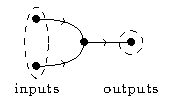
\includegraphics{InclGrphx--example--open_graph_1}
\]
Given open graphs $G$ and $G'$,
if the set of inputs in $G$
and the set of outputs in $G'$
have the same cardinality,
we can glue them together
along a bijection.
This gives a way 
to turn a pair of 
compatible open graphs
into a single open graph.  
For instance, 
to the above open graph, 
we can connect 
\[
	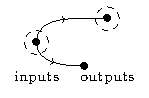
\includegraphics{InclGrphx--example--open_graph_2}
\]
to form
\[
	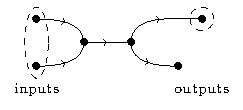
\includegraphics{InclGrphx--example--open_graph_3}
\]
We make this precise with
cospans and pushouts.

\begin{defn}
	\label{def:Open_Graph}
	Consider the functor 
		$N \colon \mathbf{FinSet}_0 \to \mathbf{Graph}$, 
	on a skeleton of $\mathbf{FinSet}$, 
	defined by the letting 
	$N(X)$ be the edgeless graph 
	with nodes $X$.  
	An \emph{open graph} is then 
	a cospan in the category 
		$\mathbf{Graph}$ 
	of the form 
		$N(X) \to G \gets N(Y)$ 
	for sets $X$ and $Y$.
\end{defn}

The left leg $N(X)$ of the cospan 
gives the \emph{input} and 
the right leg $N(Y)$ the \emph{outputs}.  
Suppose we have another open graph $G'$ 
with inputs $N(Y)$ and outputs $N(Z)$.  
Then we can compose cospans 
\[
	N(X) \to G \gets N(Y) \to G' \gets N(Z). 
\] 
by pushing out over 
$G \gets N(Y) \to G'$ to get 
\[
	N(X) \to G +_{ N ( Y ) } G' \gets N(Z).
\] 
By taking isomorphism classes 
of these pushouts, 
we obtain a category whose 
objects are those in the image of $N$ 
and morphisms are open graphs. 
But we can do better! 

Thus far, we have only 
just described the first layer 
of bicategory
introduced by the author 
under the name $\cat{Rewrite}$
\cite{Cicala_SpansCospans}.
It was shown in a joint work with Courser
\cite{CicalaCourser_BicatSpansCospan} 
that $\mathbf{Rewrite}$ is 
symmetric monoidal and compact closed. 
The monoidal structure is 
induced from the coproduct of graphs.  
Here, we take Stay's definition 
of compact closedness for bicategories
\cite{Stay_CompactClosedBicats}. 
As discussed in the introduction, 
we will work instead with
the slightly modified version of $\cat{Rewrite}$
described in Definition \ref{defn:Rewrite}.

Construction on this modified bicategory
begins with the theorem below.
First, we introduce some needed terminology.
A \emph{span of cospans} is 
a commuting diagram as illustrated 
in Figure \ref{fig:spans_of_cospans}.  
A \emph{parallel class} of spans of cospans is
formed by the equivalence relation 
given by identifying
spans of cospans
with same domain and codomain.

\begin{thm}
	\label{thm:SpCspC_is_SMCC_bicategory}
	Let $\mathbf{C} = (\cat{C}_0,\otimes,I)$ 
	be a finitely complete and cocomplete
	(braided, symmetric) monoidal category 
	such that $\otimes$ preserves colimits.   
	There is a 
	(braided, symmetric) monoidal bicategory 
	$ \spcsp{C} $ 
	whose 
	0-cells are $\cat{C}$-objects, 
	1-cells are cospans in $\cat{C}$, and 
	2-cells are	parallel classes 
	of spans of cospans.
	In case $\cat{C}$ is cocartesian, 
	then $\spcsp{C}$ is also compact closed.
\end{thm}

We prove this theorem in 
Appendix \ref{sec:SMCC_Bicat_SpCsp}. 
It follows from taking parallel classes of 
2-cells that hom-categories 
in $\spcsp{C}$ are groupoids.

Using parallel classes 
of 2-cells instead of
isomorphism classes
has several advantages.  
First, it removes two conditions 
required of $\cat{C}$
in $\bimonspcsp{C}$: 
that $\cat{C}$ be a topos and 
that the legs in the 
span of cospans be monic. 
It also allows us, 
when $\cat{C}$ is sufficiently
like $\cat{Graphs}$, 
to rewrite an edge into a node  
in analogy to deforming a 
topological string 
into a point. 
Moreover, these 2-cells
give us unitary 1-cells.

Recall that there are two ways 
to compose 2-cells in a bicategory.  
Horizontal composition in 
$\mathbf{Sp}(\mathbf{Csp}(\mathbf{C}))$ 
uses pushouts and 
vertical composition uses pullbacks:
\begin{equation}
\label{eq:Hor_and_Vert_Composition}
\raisebox{-0.85\height}{%
	\raisebox{0.3\height}{%
		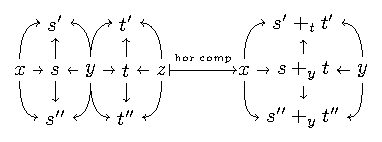
\includegraphics[scale=0.85]{InclGrphx--SpCsp--horizontal_composition} 
	}
	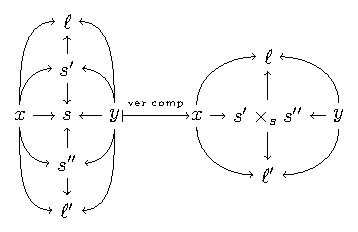
\includegraphics[scale=0.85]{InclGrphx--SpCsp--vertical_composition}
}
\end{equation}

\begin{defn}
\label{defn:Rewrite}
	Define $\cat{Rewrite}$ to be 
	the 1-full and 2-full 
	SMCC sub-bicategory of 
	$\spcsp{Graph}$ 
	whose 0-cells are 
	exactly those graphs in 
	the image of the functor 
	$N \colon \mathbf{Set}_0 \to \mathbf{Graph}$.
\end{defn}

The conceit of $\mathbf{Rewrite}$ 
is that the 1-cells are open graphs 
whose inputs and outputs are 
chosen by the $0$-cells, 
and the $2$-cells are 
rewrite rules that preserves 
the input and output nodes.
By rewrite rules, we mean those 
taken from the 
double pushout graph rewriting 
approach \cite{Corradini_AlgApprGraphTrans}.
Our open graphs are 
a different formulation
of what amounts to the same concept
explored by Dixon, Duncan, and Kissinger
	\cite{Dixon_OpenGraphs}
though we go a bit further, 
getting an SMCC bicategory
of open graphs instead of a 1-category.
 
Our motivation for constructing $\mathbf{Rewrite}$ 
is not to study it directly, 
but for it to serve 
as an ambient context in which 
to generate SMCC sub-bicategories 
on some collection of open graphs 
and rewriting rules. 
Presenting categories by
open graphs and rewrite rules
is common enough
	\cite{Dixon_OpenGraphs,Fong_AlgOpenSystems,Pollard_OpenMarkov}
to warrant finding a common
framework in which to fit such categories.
However, there are drawbacks to this approach. 
For example, working with open graphs 
is only useful to model graphical languages 
whose terms are equal 
up to ambient isotopy in $4$-space.
This limits the current approach to 
only symmetric monoidal (bi)categories 
as Selinger's work shows
	\cite{Selinger_GraphicsMonCats}.
	
Employing open graphs is 
not quite enough for us
to fully capture the zx-calculus.
We still need to color
our open graphs in a way
that corresponds to the
zx-diagram node types.

